\chapter{A data mining framework for automatic event detection and summarisation}\label{TheoreticalFramework}
\ifpdf
    \graphicspath{{Chapter2/Chapter2Figs/PNG/}{Chapter2/Chapter2Figs/PDF/}{Chapter2/Chapter2Figs/}}
\else
    \graphicspath{{Chapter2/Chapter2Figs/EPS/}{Chapter2/Chapter2Figs/}}
\fi

In this chapter, we will define a theoretical framework for construction of a 
data mining system which can extract events from Twitter data. The system comprises of a number
of individual components which when combined together construct a complete framework for 
event extraction. These components are explained in detail in the sections below and in 
Chapter \ref{chap:DesignAndImplementation} we discuss the concrete implementation of this framework as 
well as the development of a proof-of-concept application using this framework.\\
The sections of this chapter introduce the motivating work for the implementation of the system
and we also take a closer look at the concepts and key ideas that are necessary to understand the process we employ.

\section{Methodology overview}\label{MethodologyOverview}
The main idea behind our methodology for event detction is the hypothesis that similar events will be described by tweets having similar
content. Therefore, the main task in our methodology is to cluster the tweets in different groups. We further hypothesise that not all of the detected
clusters will describe real events, since clustering will detect topics such as discussions about celebrities or politicians which cannot be thought as events
accortding to our definition of an event. Having idientified some events we can then further investigate these clusters extract useful information from them which 
will serve as the event summary. The theoretical foundations of this procedure and its sub-components are described in detail in the rest of this chapter.  

\section{Raw text processing}\label{RawDataProcessing}
Mining and analysing text corpora are two well studied problems but in our case we face a slightly
different problem. Social media content and especially tweets are very short (140 characters)
and usually contain slang phrases, abbreviations and irrelevant information. Therefore, is of
foremost importance to ensure that clever data preprocessing takes place in order to help us in
the subsequent tasks. Below we describe the main steps we must follow to pre-process our raw text tweets. 

\subsection{Natural language processing}

Natural language processing (NLP) is a field of computer science and linguistics which is concerned with the extraction of information from a human language 
input. NLP is used extensively throughout this project since we deal with human generated content and we use several of its applications. NLP in the context 
of raw data processing is used to clean and normalise our initial input which is a tweet containing raw text.\\ 
Since tweets usually contain URLs and HTML code one of the first priorities is to remove these elements. Then, the following NLP algorithms
can be used on our data:

\begin{itemize}
 \item \textbf{Sentence segmentation and tokenization:} Raw text is split into sentences and then each sentence is further subdivided into words using a tokenizer. 
 \item \textbf{Stopword removal:} Some of the words occuring in the documents are common English words such as 'the', 'and' and 'a'. These words convey almost no information 
 but most importantly, they can reduce the clustering accuracy. Two documents can be erroneusly considered related if they contain common English words like the ones
  we have already mentioned. Therefore, it is important to remove these stopwords. Usually, a dictionary of the common English stopwords is used to filter them out.   
 \item \textbf{Stemming:} This is a mechanism for reducing English words to their stem form. For example, the stem form of the words `connections' and `connected' is `connect'. This mechanism is particularly useful in the field of information retrieval and indexing. M.F Porter designed the most widely used stemming algorithm in 1980 [Insert ref here]. This algorithm works by applying a set of different rules, which after a number of iteration yield the final resut which is the stem of the word. Porter
has developed 62 rules which may or may not apply to a given word.
\end{itemize}\vspace{15pt}

In section \ref{sec:SummaryGen} we explore more applications of NLP and how we can use them to extract automatic summaries, named entities or sentiment from documents.

\subsection{Inverted index}
An inverted index, also known as an inverted file, is a data structure central to text-based information retrieval. The name is derived from its 
purpose and design which is to map key-value pairs, where a key is a term in a document and the value is the list of documents that contain this term.
For example if we have two documents:\\
\emph{Document1}: The cat is on the tree. \\
\emph{Document2}: The cat sat on the mat. \\
then the inverted index will look like:

\begin{center}
\begin{tabular}{ |l | l| }
  \hline
  \textbf{Key} & \textbf{Value} \\ \hline
  the & \{Document1, Document2\} \\
  cat & \{Document1, Document2\} \\
  is & \{Document1\} \\
  on & \{Document1, Document2\} \\
  tree & \{Document1\} \\
  sat & \{Document2\} \\
  mat & \{Document2\} \\
  \hline
\end{tabular}
\end{center}

The main reason for using an index is to increase the speed and efficiency of searches of the document 
collection. In our system the inverted index is vital component since it allows us to construct
term-documment vectors easily and also filter terms and documents. For example, using our index we
can find the words that appear either too often or less frequently and filter them out. This is used
to reduce the dimensionality of our dataset by removing unneccesary words. Alternatively, we
can remove documents/tweets which contain keywords that appear too often or less frequently.

\section{Cluster Analysis}

Cluster analysis is the process of grouping a set of data objects into multiple clusters where all the
objects in a cluster have high similarity but they are very dissimilar to objects in other clusters. The set
of clusters resulting from a cluster analysis can be referred to as a clustering. Clustering is an unsupervised 
learning method since deals with finding a structure in a collection of unlabeled data. Figure 3.3 depicts a simple 
clustering example where a clustering algorithm is applied on an unlabeled dataset and four different clusters are detected.\\
Cluster analysis is applied in a wide range of applications such as business intelligence, image pattern recognition, biology and 
security. In our project we are interested in cluster analysis and its application in document clustering. We would like to cluster tweets 
which are similar in terms of both textual content and describe the same topic.\\
In the rest of this section we describe the key ideas behind document clustering and we explain the main clustering algorithms that
will be used in our implementation.

\begin{figure}[!htbp]
  \begin{center}
    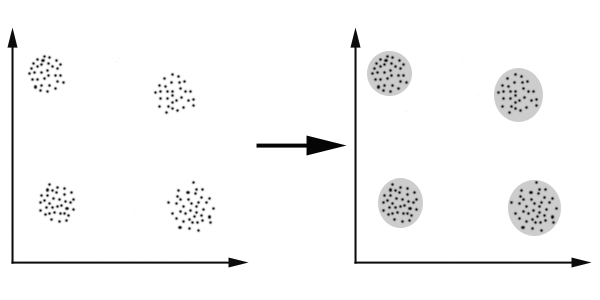
\includegraphics[height=1.5in, width=4in]{clustering}
    \caption{The result of appplying a clustering algorithm to unlabeled data. Four distinct clusters have been detected.}
    \label{ClusteringExample}
  \end{center}
\end{figure} 

\subsection{Vector space representation}

Document need to be preprocessed in order to be in a form that will allow us to perform clustering. 
The most common approach is to use the vector space representation model. The vector space representation transforms the 
documents into vectors of term frequencies which can then be used as a means to assess the similarity between documents.\\
We can represent each document in a dataset by a vector of identifiers. Usually, these identifiers are the distinct words in the document and 
the resulting vector is called term-frequency vector. If we combine all the vectors for the documents in our dataset we will end up with an 
\boldmath $m \times n$  \unboldmath  matrix \boldmath $A$ \unboldmath. Each of the $m$ documents in the document collection are assigned a row 
in the matrix, while each of the $n$ unique terms in each document are assigned a column in the matrix. A non-zero element $a_{ij}$ in \boldmath 
$A$ \unboldmath, indicates not only that term $j$ occurs in document $i$, but also the number of times the term appears in that document. Since the number of terms in a given 
document is typically far less than the number of terms in the entire document collection, A is usually very sparse.\\
For example in Table 3.1 we see that $Document1$ contains three instances of the word team, while football occurs five times. We can also infer that
the words ball and world are missing for the entire document, as indicated by the value of zero at those entries of the matrix.\\  
The main advantage of transforming the documents in the vector space is that we can define vector-space similarities between documents and therefore
we can apply clustering algorithms on the document collection. In section we provide a more detailed discussion on similarity metrics and the vector space 
representation is used in clustering documents.

\begin{table}[tbp]
\centering
\begin{tabular}{ l  l  l  l  l  l  l }
  \hline
  \textbf{Document} & \textbf{team} & \textbf{ball} & \textbf{football} & \textbf{countries} & \textbf{world} & \textbf{england} \\ \hline
  \emph{Document1} & 3 & 0 & 5 & 1 & 3 & 1 \\
  \emph{Document2} & 2 & 1 & 2 & 0 & 8 & 2\\
  \emph{Document3} & 1 & 5 & 3 & 0 & 1 & 3\\
  \emph{Document4} & 5 & 0 & 1 & 2 & 5 & 4\\
  \hline
\end{tabular}
\caption{Term-frequency vector representation of documents}
\label{termfrequencyTable}
\end{table}

\subsection{Assigning weights to terms with TF-IDF weighting}
Once a document is transformed in its term-frequency vector we can assign weights to each term in the vector. So far the term-frequency vectors treat 
all the terms as equal but this may not be the case. For example, a word that appears more frequently than others in a document could be considered as an 
important word. At the same time words that appear frequently in the corpus, such as 'a', 'the', 'and', are not very useful and their 
importance must be discounted. \\
The most common method to solve this problem is the TF-IDF weight (TF-IDF stands for term frequency-inverse document frequency) which quantifies the importance of a term in a document of a document collection. More specifically, the more a word occurs in a document, and the less it occurs in the rest of the coprus, the higher its TF-IDF weighting 
will be. Mathematically, TF-IDF is expressed as:\\
\begin{eqnarray}
tf-idf_{t,d} = tf_{t, d} \times idf_t
\end{eqnarray}

where $tf_{t, d}$ is the importance of term $t$ in document $d$ and $idf_t$ is the importance of term $t$ relative to the entire corpus. $tf_{t,d}$ is higher when the term occurs many times in the document and $idf_t$ is higher when it occurs rarely in the dataset. Therefore, the TF-IDF weighting for a term is very high if the term occurs frequently in a single document but very rarely in the entire corpus and it is low when the term either occurs rarely in a document or frequently in the entire corpus. TF-IDF is widely used to compare the similarity between documents and a common use case is for search queries where the similarity of a query $q$ with a document $d$ is calculated using TF-IDF, providing
a sorted list of the most relevant documents. 
\\
   
\subsection{Feature selection}
TODO: Discusss feature selection methods used in our system.

\subsection{Distance measures}
In data mining applications including clustering we must decide whether two objects are similar or dissimilar. In document clustering we wish to 
assess how similar are two documents in comparison to one another. Based on the similarity between two objects we can make the decision whether to
group them in the same cluster or not. In this section we present three commonly used similarity measures which will be used throughout our work. 

\subsubsection{Euclidean distance}
Euclidean distance is probably the most popular distance measure and can be thought as the straight line connecting the two data points that we try to compare.
Let the two data points be $i = (x_{i,1}, x_{i,2},...,x_{i,p})$ and $j = (x_{j,1}, x_{j,2},...,x_{j,p})$ where $p$ is the number of the numeric attributes. The Euclidean distance between $i$ and $j$ can then be defined as:\\
\begin{eqnarray}
d(i,j) = \sqrt{(x_{i,1} - x_{j,1})^2 + (x_{i,2} - x_{j,2})^2 + ... +(x_{i,p} - x_{j,p})^2 }
\end{eqnarray} 

Euclidean distance is the default distance measure used with the k-Means algorithm. 

\subsubsection{Cosine similarity}
The similarity of two documents which are represented as term vectors, corresponds to the correlation between the vectors. This is calculated as the cosine of the
angle between vectors, the so-called cosine similarity. Cosine similarity is widely used for text documents and especially in clustering documents. Let $x$ and $y$ be 
two vectors for comparison. Cosine similarity is defined as:

\begin{eqnarray}
sim(x,y) = \frac{x \cdot y }{\norm{x} \norm{y}} 
\end{eqnarray} 

where $\norm{a}$ is the Euclidean norm of vector $a$. This measure computes the cosine of the angle between the vectors x and y with a cosine value of $0$ meaning that the two vectors are at 90 degrees to each otther and therefore are not a match. If the cosine value is $1$ then the two vectors are identical and they are a perfect match. 

\subsubsection{Jaccard coefficient}
The Jaccard coefficient measures similarity as the intersection divided by the union of the objects. For text document, the Jaccard coefficient compares the sum weight of shared terms to the sum weight of terms that are present in either of the two document but are not the shared terms.

\begin{eqnarray}
sim(i,j) = \frac{q}{q + r + s}  
\end{eqnarray} 
where $q$ is the number of variables that are positive for both objects, $r$ is the number of variables that positive for $i$ and negative for $j$ and $s$ is the  number of variables that are positive for the $j$ and negative for $i$.


\subsection{Clustering methods}
There are many clustering algorithms and usually the belong to one of the following categories, as they are described in [put reference to the book]:

\begin{itemize}
 \item \textbf{Partitioning methods:} Partiotioning methods operate on a number of data points and form partitions of the data where each partition is a cluster. Usually, these methods have the restriction that each object must belong to a single cluster. They are only effective for a small to medium datasets. 
 \item \textbf{Hierarchical methods:} A hierarchical method creates a hierarchical decomposition of the given set of data objects. These methods can be firther subdivided 
 in agglomerative and divisive, based on how the decomposition is formed. Hierarchical methods suffer from the fact that erroneous merges or split cannot be undone. 
 \item \textbf{Density-based methods:} These methods, unlike most other techniques, can find clusters of arbitrary shapes. They can do so by employing the notion of density. The
 main idea is to keep growing a cluster as long as the density of a 'neighborhood' exceeds some threshold. Therefore, clusters are dense regions of data points that are separated 
 by low-density regions.
 \item \textbf{Grid-based methods:} Grid-based methods quantize the space into a number of cells which form a grid structure, All the clustering operations are performed on the grid structure. Since the provessing time is only dependent on the number of cells and not the number of data points these methods have fast processing time. 
\end{itemize}\vspace{15pt}

Below we outline the basic clustering methods that will be used in our system and we look into their key ideas that will guide 
our implementation. 

\subsubsection{k-Means algorithm}
k-Means algorithm belongs to the partioning methods category. A partitioning method distributes the objects in $D$  into k clusters, $C_1, ..., C_k$, such that $C_i \subset D$ and $C_i \cap C_j = \emptyset$ for $(1 \leq i, j \leq k)$. k-Means is a centroid-based technique whic means that a cluster, $C_i$, is represented by a centroid which can be the mean of all the points in the cluster. Practically, this representation is the centre point of the cluster. \\
More specifically, the k-Means algorithm starts by randomly selecting k of the object in D, and each one represents a cluster centre. Then for each of the remaining objects in D, the algorithm calculates the distance between each of the k cluster centres. The closest cluster is selected and that point is assigned to this cluster. The mean of each cluster is re-calculated after a new point has been assigned to it. At this point the k-Means algorithm iteratively tries to improve the within cluster variation (improving an objective function) by reassigning all the objects according to the new cluster centres. The algorithm continues until it converges to the point where the clusters formed in the previous iteration are the same to the clusters formed in this iteration. Figure 3.4 (TODO:Put image ref) depicts a simple example of the k-Means algorithm with two clusters. In the first image, the two centroids, which are depicted as dark circles are initialised to a random position in the space. In the second image each of the data points is assigned to the nearest centroid and in this case A and B are assigned to the top centroid and C, D, and E are assigned to the bottom centroid. In the third image, each centroid's average is re-calculated and moved to its new position. When the assignments are calculated again, it turns out that C is now closer to the top centroid, while D and E remain closest to the bottom one. Thus, the final result is that A, B, and C belong in one cluster, and D and E in the other. \\

\begin{figure}[!htbp]
  \begin{center}
    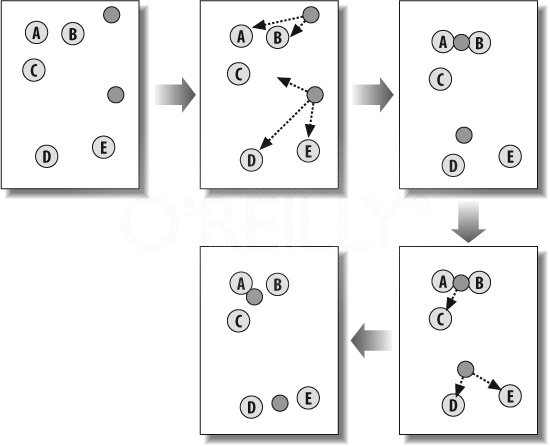
\includegraphics[height=2.5in, width=4in]{kmeans-example}
    \caption{k-Means clustering with two clusters}
    \label{kMeansExample}
  \end{center}
\end{figure} 
 
The algorithm is not guaranteed to converge to a global optimum and the results depend on the initial allocations of the k centres. The time complexity is $O(nkt)$ where n is the total number of of objects, k is the number of clusters and t is the number of iterations. Therefore, the k-Means algorith is relatively scalable. 

\subsubsection{DBSCAN algorithm}
k-Means algorithm and hierarchical clustering algorithms are very good at clustering spherical-shaped clusters. However, they are not able to detect clusters of arbitrary shape such as the one below.  \

\begin{figure}[!htbp]
  \begin{center}
    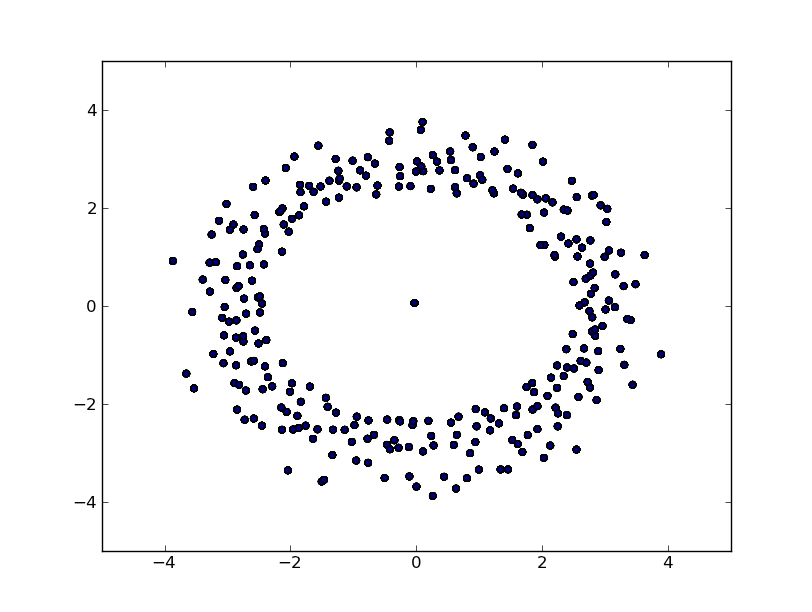
\includegraphics[height=3in, width=4in]{dbscan-example}
    \caption{The DBSCAN algorithm belongs to the density-based methods which can find clusters of arbitrary shapes (not only spherical).}
    \label{DBSCANExample}
  \end{center}
\end{figure} 

In order to alleviate the problem one have to look into density-based clustering algorithms. These algorithms model clusters as dense regions in the data space. One of the most popular algorithms of this kind is the Density-Based Clustering Based on Connected Regions with High Density (DBSCAN). \\ 
DBSCAN defines density of an object $o$ as the number of objects close to $o$. DBSCAN finds core objects which are objects with dense neighborhoods. Then it connects those core objects and their neighborhoods to form clusters. In order to assess density, DBSCAN uses a constant $\epsilon  > 0$ which defines the radius of the neighborhood of an object $o$ and then finds the number of objects in the neighborhood. If the number is above a threshold $MinPts$ then the neighborhood is considered dense. Given a set, $D$, of objects, we can identify the core objects using $\epsilon$ and $MinPts$. The problem of clustering then reduces to the task of finding dense regions using the core objects and their neighborhoods. \\\\
The complexity of the algorithm in our implementation is $O(n^2)$ but it can be reduced to $O(n\log n)$ if a spatial index is used. This means that this algorithm doesn't allow us to scale it up to large volume of data. The main disadvantage of the DBSCAN algorithm is that the user has to pass the $\epsilon $ and the $MinPts$ parameters which usually is a difficult task and some datasets are very sensitive to variations of these parameters. 

\subsubsection{Non-negative matrix factorisation algorithm}
Non-negative matrix factorization (NMF) is not a clustering algorithm per se but it can be shown that it is equivalent to a relaxed form of k-Means algorithm. This algorithm takes as input the term-document matrix, constructed during clustering pre-processing and decomposes it into two other matrices. The first one is a feature-term matrix (or features matrix) and the other a document-feature matrix (or weight matrix). In the latent semantic space derived by the NMF, each axis captures the base topic of a particular document cluster, and each document is represented as an additive combination of the base topics. The cluster membership of each document can be easily determined by finding the base topic (the axis) with which the document has the largest projection value. The only constraint of the algorithm is that the two derived matrices should be non-negative.\\\\ 
In the context of document clustering we use matrix factorisation to reduce a large set of documents to a smaller set that captures their common topics (features) [put ref to the book Collective Intelligence ]. We start with a term-frequency matrix and we wish to factorise this matrix to get the two matrices we mentioned above. The features matrix has a row for each feature and a column for each term (word). An example of such a matrix is shown below. The values indicate how important a word is to a feature. Each feature represents a topic that is implied from a set of documents. 

\[
\bordermatrix{~ & football & ball & england & newspaper \cr
                  feature 1 & 1 & 0 & 3 & 2 \cr
                  feature 2 & 0 & 1 & 3 & 1\cr
                  feature 3 & 0 & 2 & 2 & 1\cr}
\]\\
The weights matrix maps the features to the documents. It has a row for each document and a column for each feature. The values indicate how much each feature matches to each document. An example of the weights matrix is shown below. 

\[
\bordermatrix{~ & feature 1 & feature 2 & feature 3\cr
                  Document 1 & 1 & 5 & 3\cr
                  Document 2 & 3 & 1 & 1\cr
                  Document 3 & 0 & 2 & 3\cr}
\] \\
The original matrix can be reconstructed by multiplying the weights matrix by the features matrix, although the resulting matrix would not be an exact reconstruction of the original one but an approximation. 

\subsubsection{Online clustering algorithm}
All the algorithms described above operate on the whole dataset, $D$, and sometimes this is not desirable or not even neccessary. Especially if the dataset is too large and we are concerned about performance and scalability. Therefore, a family of algorithms have been studied in order to modify common algorithms for scalability. These algorithms are called sequential or online clustering algorithms. By online in this context we mean an algorithm that does not keep all the data objects in memory at the same time, but processes them sequentially, keeping only a subset if them.\\
Suppose we are given a sequence of N tweets $T = {t_1, ..., t_N}$ where each $t_i$ is a vector of $a$ attribute values, and we want to split them into $K$ clusters. Each cluster is described by a prototype vector $p_i = {p_1, ..., p_f}$ where $i = 1, ..., K$. Given that the task of finding good clusters is to minimize an objective distance function $J$ the algorithm works as follows:
\begin{enumerate}
   \item Pick the next example in the sequence T
   \item Compute the distances from this example to all the cluster prototypes and pick the minimum one.
   \item Update the prototype vector in order to come closer to the current example  
   \item Goto step 1  
 \end{enumerate} 
 
The implementation of our online algorithm is based on the work proposed in the paper "Improving the Robustness of ‘Online Agglomerative Clustering Method’ Based on Kernel-Induce Distance Measures" by Zhang et al. They have used kernel-functions for distance measures and post-processing filtering is performed to remove noise from data. Extending their work, in our implementation we have tried to increase its scalability by allowing only a sliding window of $n$ tweets to be in memory each time when the term-document vectors are calculated. 

\section{Automatic text summaries}\label{SummaryGen}

Another integral component of our framework is the module repsonsible for generating automatic summaries of the events. In Chapter \ref{chap:Introduction}
we described the problem of event summarisation as the task that will extract the top tweets for an event that are most helpful for a human to understand the event.
The term 'helpful' is vague and therefore we have defined three criteria, described in [TODO: put ref for the paper Selecting Quality Twitter Content for Events ] that will evaluate qualitatively our summaries and guide our implementation choices. The three criteria are:

\begin{itemize}
 \item \textbf{Quality:} It refers to the textual quality of the messages, which reflects how well they can be understood by a human.
 \item \textbf{Relevance:} It refers to how well a Twitter message reflects information related to its associated event.
 \item \textbf{Usefulness:} It refers to the potential value of a document for someone who is interested in learning more about an event.
\end{itemize}\vspace{15pt}

\subsection{Generating automatic document cluster summaries}
In general, in automatic text summarisation we are interested in generating a shortened version of a large corpus or document but maintaining the integrity and meaning of 
the original text. There are to variations of the automatic text summarisation: the extractive summarisation method which produces summaries by choosing a subset of the sentences
in the original document or documents and abstractive summarisation, where the information in the text is rephrased.\\\\
In our case the task is to reduce a large set of tweets in a smaller subset by ranking the individual tweets in a subset and selecting the top ranking ones.
In our project we consider two methods extractive summarisation methods, the centroid-based summarisation and the LexRank algorithm.

\subsubsection{Centroid-based summarisation}
The centroid similarity approach computes the similarity of each message to its associated event cluster centroid. The cluster centroid is calculated by averaging the weight across all the document TF-IDF weigthed term-frequency vectors in a specific event. The method then selects the documents with the highest similarity value. The implicit assumption is that a cluster’s centroid emphasises important terms which are relevant to the event. For example a cluster describing the topic of some protesters giving flowers to policemen in Cairo would give higher weight to the terms "protesters", "flowers" and "policemen". Therefore documents with high similarity to these key terms are more likely to reveal key aspects of the event which is highly desired by the relevance and usefulness goals. Additionally, the quality criterion is satisfied since the centroid weights are based on frequency across all messages, and therefore they contain no typos or spelling mistakes (which can greatly affect the quality of a document). 

\subsubsection{LexRank algorithm}
The idea of the LexRank algorithm was proposed by [put ref to paper here] and it was successfully used for extractive summarisation tasks. Instead of the idea of a centroid LexRank uses the notion of centrality, which
assumes that sentences which are similar to many other sentences in a cluster indicate "topicality". That is, the
sentence that is the most similar to other sentences is the most topical. LexRank conceptualises sentences to be forming a graph which has the sentences as nodes and the edges indicate which sentences are similar (if the similarity is above a threshold we add an edge between two nodes). The sentence/node with the more edges has the higher centrality. Usually the cosine similarity measure is used for this purpose. Other methods such as degree centrality consider each edge as being an equal vote for centrality and therefore the most edges a node has the highest the centrality. However, LexRank takes a slightly less democratic approach by giving "prestigious" sentences more voting power. The higher the centrality of a node the more its vote counts. A way of formulating this idea is to distribute the centrality of a node to its neighbors. This can be formulated by:

\begin{eqnarray}
L(u) = \sum_{v \in adj[u]}^{\infty}\frac{L(v)}{deg(v)}
\end{eqnarray} 
where $L(u)$ is the centrality of node $u$, $adj[u]$ is the set of nodes adjacent to $u$, $deg(v)$ is the degree of node $v$.

In order to ensure that a "random walker" is not stuck during a walk in the graph we need to introduce a damping factor $d$ which was first introduced by Page et al. (1998) in order to solve this problem. The equation for LexRank then becomes:

\begin{eqnarray}\label{LexRankEquation}
L(u) = \frac{d}{N} + (1-d) \sum_{v \in adj[u]}^{\infty}\frac{L(v)}{deg(v)}
\end{eqnarray} 
where N is the total number of nodes in the graph. The above equation is called the LexRank equation and is defined in a recursive manner, and can be computed via an iterative routine called the power method (the algorith is given in Chapter \ref{DesignAndImplementation}). This is essentially the same as the PageRank algorithm which is the backbone of the Google search engine with the only difference that the edges are undirected since the cosine similarity is a symmetric relation.

\subsection{Detecting named entities and locations in documents}
The summaries produced by the algorithms described above are a good representation of the event and can help a human to understand the event. However, sometimes some additional
information is needed to comprehend an event. In Chapter \ref{chap:Introduction} we described an event as a collection of attributes such as keywords, geographic location and entities involved. Therefore, we wish to be able to automatically extract these attributes for an event and included them in the summary of an event. The keywords describing the event are simply the words having the highests weight in an event cluster and can extracted very easily. For the named entities and locations we have to use a technique called named entity extraction which is part of the NLP algorithms. The method takes as input a piece of text and locates and classifies atomic elements in text into diffeent categories such as the names of persons, organisations and locations.


\section{Twitter user classification}
Different types of users interact and disseminate information daily on Twitter. Depending on the type of user we expect the content of a tweet to vary and consequently the quality of a tweet will vary too. For example renowned journalists are more likely to produce high quality tweets which easily be trusted as a reliable source of information. On the other hand tweets generated by a tweet bot might be considered unreliable since bots are known to release rumors. Therefore, it is crucial to be able to distinguish different types of users in order to ensure that we will extract high quality events that provide useful information and not just rumors. Additionally, it is interesting in its own right to investigate what is the distribution of the users tweeting for an event. For example, we would like to find out whether activists can start and sustain an event discussion online or whether celebrities or political figures can spark the interest of other Twitter users. In order to do that we need to find a way to classify users.\\\\ 
Classification is the process of finding a model that describes and classifies data classes. The model is derived based on a set of training data (data objects which their class labels are known). Then the derived model is used to predict the class of an uknown instance which is presented to the learning system.    

\subsection{Decision trees}
Decision Tree learning is a method for approximating discrete classiffication functions using a tree-based representation. We can make use of this method to inductively infer [put ref here] unknown relations within our dataset. A nice property of the decision trees is that they can also be represented as a set of if-then rules, therefore the task of interpreting them is an easy task for a human. A learned decision tree is able to classify a new instance by sorting it down the tree to the appropriate leaf node, then returning the classification associated with this leaf. Every node in the tree tests some attribute value of each new instance, and the branches of each node represent a possible value for that attribute.\\\\
Figure 3.6 illustrates a simple decision tree, which classifies a day's weather conditions according to wether they are suitable for playing tennis [put ref to mitchell's book]. If the decision tree is presented with an example of a day when the outlook is sunny, the temperature is hot, the humidity is high and the wind is strong then this example would be sorted down the leftmost branch and therefore would be classified as negative, i.e, this day is not suitable for playing tennis. Alternatively, the tree could be represented as if-then rules:\\  


\begin{center}
  (Outlook = Sunny $\wedge$ Humidity = Normal)\\
  $\vee$ (Outlook = Overcast)\\
  $\vee$ (Outlook = Rain $\wedge$ Wind = Weak)
\end{center}

\begin{figure}[!htbp]
  \begin{center}
    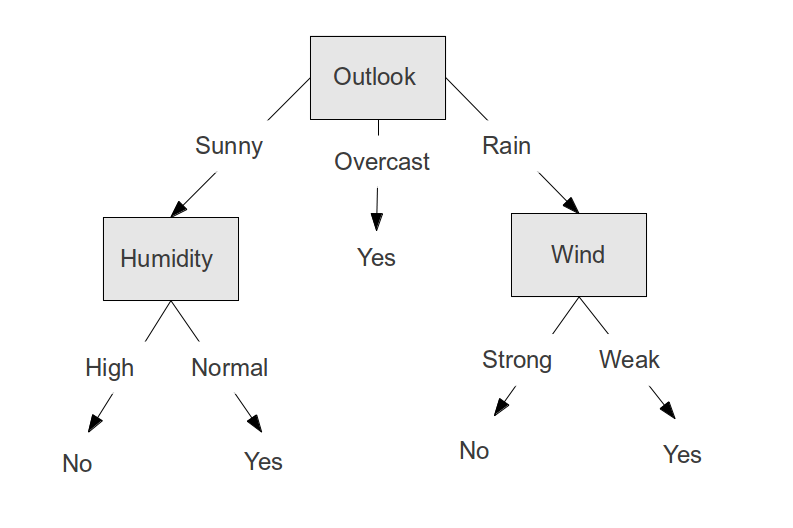
\includegraphics[height=2in, width=4in]{decision-tree-example}
    \caption{A simple decision tree.}
    \label{DecisionTreeExample}
  \end{center}
\end{figure} 

\subsection{Neural networks}
[TODO explain Neural Nets]

\section{Summary}

Show a simple diagram with a lot of tweets becoming vectors and then those becoming clusters and then some of them events.
This is the outout of the algorithm.

% ------------------------------------------------------------------------

%%% Local Variables: 
%%% mode: latex
%%% TeX-master: "../thesis"
%%% End: 
